\documentclass[10pt]{article}
%Formato extenso:report
\begin{sloppypar}
	
\end{sloppypar}
%Formato corto:article

% Esto es para que el LaTeX sepa que el texto esten espanol:
\usepackage[spanish]{babel}

% Esto es para poder escribir acentos directamente, no recomendable si trabaja en varios sistemas operativos:
%\usepackage[ansinew]{inputenc}    % Windows: Descomentar si quiere escribir con acentos directamente
% \usepackage[latin1]{inputenc}         % Linux: Descomentar si quiere escribir con acentos directamente
%\usepackage[applemac]{inputenc} % MacOS: Descomentar si quiere escribir con acentos directamente

% Paquetes de la AMS:
\usepackage{amsmath, amsthm, amsfonts,amssymb}

% Borrame si quieres:
\usepackage{multicol}

% Referencias
\usepackage{hyperref}

% Paquete para escribir codigo
\usepackage{listings}
\lstset{basicstyle=\footnotesize\ttfamily,breaklines=true}
\usepackage{alltt}

% Paquete para incluir imagenes
\usepackage{graphicx}

% Paquete para incluir varias imagenes en una
% \usepackage{subfig}#subfig deprecated?
\usepackage{caption}
\usepackage{subcaption}

% para poder fijare las imagenes ([H])
\usepackage{float}

% para agregar opciones al enumerate
\usepackage{enumerate}


% Teoremas
\newtheorem{thm}{Teorema}[section]
\newtheorem{cor}[thm]{Corolario}
\newtheorem{lem}[thm]{Lema}
\newtheorem{prop}[thm]{Proposici\'on}
\theoremstyle{definition}
\newtheorem{defn}[thm]{Definici\'on}
\theoremstyle{remark}
\newtheorem{rem}[thm]{Observaci\'on}
\theoremstyle{definition}
\newtheorem{prob}{Problema}

% Calculus symbols
\newcommand{\pd}[2]{\frac{\partial #1}{ \partial #2}}   % First partial derivative command
\newcommand{\td}[2]{\frac{\mathrm{d} #1}{ \mathrm{d} #2}}
\newcommand{\pdd}[2]{\frac{\partial^2 #1}{ \partial #2 ^2}}   % Second partial derivative command
\newcommand{\pddc}[3]{\frac{\partial^2 #1}{ \partial #2 \partial #3}}   % Second partial derivative command

% Continuum mechanics & FEM symbols
\def\sca   #1{\mbox{\rm{#1}}{}}
\def\mat   #1{\mbox{\boldmath $\mathsf #1$}}
\def\vec   #1{\mbox{\boldmath $#1$}{}}
\def\ten   #1{\mbox{\boldmath $#1$}{}}
\def\ltr   #1{\mbox{\sf{#1}}}
\def\bltr  #1{\mbox{\sffamily{\bfseries{{#1}}}}}

% math operators and symbols
\DeclareMathOperator{\dive}{div}
\DeclareMathOperator{\trace}{trace}
\DeclareMathOperator{\tr}{tr}
\DeclareMathOperator{\symm}{symm}
\DeclareMathOperator{\sk}{skew}
\DeclareMathOperator{\grad}{grad}
\DeclareMathOperator{\Grad}{Grad}
\DeclareMathOperator{\curl}{curl}
\DeclareMathOperator{\Curl}{Curl}
\def\R{\mbox{\(\mathbb{R}\)}}
\def\dx{\mbox{\(\,\mathrm{d}x\)}}



% Page margins
%\topmargin=-2cm
%\textheight=22cm
%\textwidth=17cm
%\oddsidemargin=0cm
\usepackage{geometry}
\geometry{left=2.5cm, right=2.5cm, top=2cm, bottom=3cm}

\begin{document}
%   \input{template.tex}
  \begin{titlepage}
    \begin{figure}
      \begin{minipage}{2.5cm}
	
\includegraphics[width=0.8\textwidth]{./figuras/LogoUC-BN}
      \end{minipage}
      \begin{minipage}{14.5cm}
	\vspace{4mm}
	{\sc PONTIFICIA UNIVERSIDAD CAT\'OLICA DE CHILE}\\
	Escuela de Ingenier\'ia\\
	Departamento de Ingenier\'ia Estructural y Geot\'ecnica\\
	{\bf ICE 3233 Elementos Finitos}\\
	\vspace{0mm}
	\hrulefill
      \end{minipage}
    \end{figure}
    \phantom{""}\vspace{60mm}

    \begin{center}
      \Huge{\textbf{Avance de proyecto \\ Elementos Finitos}}\vspace{95mm}\\
      \raggedleft \Large{Jos\'e Galaz \\ Jaime Soto \\ \today\\ 
    \end{center}
  \end{titlepage}
  
  \section{Introducci\'on}
    La intro es complicada....
  \section{Deducci\'on de la formulaci\'on fuerte y planteamiento del problema}
    Sea  $\Omega' \subset \mathbb{R}^3$ el dominio de inter\'es, $t_f>0$ el tiempo final de la simulaci\'on,   $\vec v : [0,t_f]\times \Omega' \rightarrow  \mathbb{R}^3$ el campo de velocidad, y $p : [0,t_f] \times \Omega' \rightarrow \mathbb{R}$ el campo de presiones, de un fluido incompresible con densidad $\rho \in \mathbb{R}^+$, que escurre sobre un fondo (topograf\'ia - batimetr\'ia) de forma dada por $b:\Omega' \rightarrow \mathbb{R}$. Si se desprecian efectos disipativos y se consideran fuerzas de volumen $\vec f_b = (0,0,-g)^T$, con $g$ la aceleraci\'on de gravedad, las ecuaciones de Navier-Stokes son \cite{toro}
\begin{align}
  \begin{split}
    \nabla \cdot \vec v &= 0 \\
    \frac{\partial }{\partial t}\vec v + \nabla \cdot \vec v \otimes \vec v  &= -\frac{1}{\rho}\nabla p + \vec f_b    \\
    v_3|_{z=\eta	} &= \frac{\partial \eta}{\partial t}+(\vec v \cdot \nabla )\eta \\
    v_3|_{z=b} &= \frac{\partial b}{\partial t} + (\vec v \cdot \nabla )b \\    
    p|_{z = \eta} &= 0
  \end{split}  
  \label{NS-incompresible}
\end{align}

En particular, en una bah\'ia de interior $\Omega \subset \mathbb{R}^2$, con borde impermeable $\partial\Omega_h$ y linea nodal $\partial \Omega_g$ tales que $\partial \Omega = \partial \Omega_h \cup \partial \Omega_g$ , y bajo el supuesto que las ondas son suficietemente largas, de forma que las aceleraciones verticales no tienen influencia significtiva sobre el perfil de presiones hidrost\'atico, y por medio de integraci\'on vertical entre el fondo $b$ y la superficie libre $\eta$, las Ecuaciones No Lineales de Aguas Someras (Non-Linear Shallow water Equations, NSWE) son, 

\begin{align}  \begin{split}
\frac{\partial}{\partial t}\left(\eta\right)+\frac{\partial}{\partial x}\left(hu\right)+\frac{\partial}{\partial y}\left(hv\right) & =0  \text{       si } x \in \Omega\\
  \frac{\partial}{\partial t}\left(hu\right)+\frac{\partial}{\partial x}(hu^{2}+\frac{1}{2}gh^{2})+\frac{\partial}{\partial y}(huv) & =-gh\frac{\partial}{\partial x}b  \text{   si } x\in\Omega\\
  \frac{\partial}{\partial t}\left(hu\right)+\frac{\partial}{\partial x}(huv)+\frac{\partial}{\partial y}(hv^{2}+\frac{1}{2}gh^{2}) & =-gh\frac{\partial}{\partial y}b  \text{     si } x \in \Omega\\
  (hu,hv) \cdot \vec n &= 0  \text{ si    } x\in\partial \Omega_h \\
   \eta &= 0  \text{ si    } x \in \partial \Omega_g  
  \end{split}
  \label{eq:nswe_cart}
  \end{align}
donde, viendo la figura \ref{fig:vars}, $h:(t,x,y) \in [0,t_f] \times \Omega \to \eta(t,x,y)-b(x,y) \in \mathbb{R}^+$ es la altura de la columna de agua,  y $(u,v)$ las componentes de velocidad horizontal promediadas en la vertical, dadas por
 $$
  (u,v)=\frac{1}{h}\int_{b}^\eta (v_1,v_2)dz
 $$
  
  \begin{figure}
    \centering
    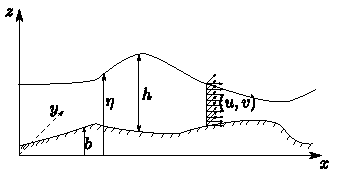
\includegraphics[width=10cm]{figs/variables.pdf}    
    \caption{ Vist esquem\'tica de ls varibles hidrodin\'amicas definidas para las Ecuaciones No Lineales de Aguas Somers (NSWE).}
    \label{fig:vars}
  \end{figure}

Las ecuaciones en \eqref{eq:nswe_cart}, forman un sistema hiperb\'olico de ecuaciones diferenciales parciales no lineales, que admite ondas de choque e interfaces seco-mojado, cuando $h$ tiende a $0$. Sin embargo, es posible obtener una linealizaci\'on del sistema \eqref{eq:nswe_cart} si se consideran peque\~nas perturbaciones a una masa de agua en reposo, es decir si
$$
	\eta=h_0+\eta' \hspace{.5cm} u=0+u',\hspace{.5cm} v = 0 + v'
$$
donde la notaci\'on $\square'$ indica peque\~nas perturbaciones sobre $\square$, y $h_0:\Omega\rightarrow \mathbb{R}$ representa la altura de la columna de agua, de forma que  \footnote{Aqu\'i el lector debe notar que este supuesto es equivalente a asumir que las ondas son de amplitud peque\~na.}
$$\left|\frac{\eta'(t,x,y)}{h_0(x,y)}\right|<<1$$
para cualquier $(t,x,y) \in [0,t_f]\times\Omega$. Bajo estos supuestos, se deducen las Ecuaciones Lineales de Aguas Someras (LSWE), dadas por
\begin{align}
	\begin{split}
	\frac{\partial \eta'}{\partial t}+\frac{\partial h_0u'}{\partial x}+\frac{\partial h_0v'}{\partial y} = 0  \text{ si } x \in \Omega\\
    \frac{\partial u'}{\partial t} + g\frac{\partial \eta'}{\partial x}=0  \text{ si } x \in \Omega\\
    \frac{\partial v'}{\partial t} + g\frac{\partial \eta'}{\partial y} = 0  \text{ si } x \in \Omega \\
    (h_0u',h_0v') \cdot \vec n = 0 & \text{ si } x\in\partial \Omega_h \\
   \eta' = 0  \text{ si } x \in \partial \Omega_g  
    \end{split}
    \label{swe}
\end{align}

    Si ademas $\eta',u',v' \in \mathcal{C}^2(\Omega)$, multiplicando la segunda y tercera ecuaci\'on de \eqref{swe}, por $h$ y derivando respecto a $x$ e $y$ es cierto que 
    \begin{equation}
    	\begin{split}
    	\frac{\partial^2 \eta}{\partial t^2} - \nabla \cdot( gh \nabla \eta) = 0, \text{ si } x \in \Omega \\
        \frac{\partial \eta}{\partial \vec n} = 0 \text{ si } x \in \partial \Omega_h \\
        \eta = 0 \text{ si }x \in \partial \Omega_g
        \end{split}
     \label{eqonda}
    \end{equation}

    donde se cambi\'o de notaci\'on al usar $\square$ como $\square'$. Las ecuaciones \eqref{eqonda} corresponden a la ecuaci\'on lineal de onda,  de celeridad $c=\sqrt{gh}$, revelando la similitud entre la propagaci\'on de ondas de amplitud peque\~na en una bah\'ia, con la de ondas ac\'usticas o el\'asticas lineales.
    
    Finalmente, si se estudian ondas estacionarias, es posible separar variables y escribir (abusando de notaci\'on en $u$), con $u:\Omega \rightarrow \mathbb{R}$
    \begin{equation}
    	\eta(t,x,y) =Re\left\{ u(x,y) e^{-i \omega t}\right\}
    \end{equation}
    
    lo cual, sustituyendo en \eqref{eqonda}, conduce a 
    
    \begin{equation}
      \begin{split}
    	\nabla \cdot \left( gh_0 \nabla u\right) + \omega^2 u = 0 \text{ si } x \in \Omega\\
        \frac{\partial u}{\partial \vec n} = 0 \text{ si } x \in \partial \Omega_h \\
        u = 0 \text{ si } x \in \partial \Omega_g
      \end{split}
        \label{helmholtz}
    \end{equation}
    
    El sistema \eqref{helmholtz} es m\'as conocido como la Ecuaci\'on de Helmholtz, y denota un problema de valores y vectores propios del operador diferencial de la ecuaci\'on de Poisson ($\nabla \cdot c^2 \nabla \square$). Es posible demostrar \cite{nica2011}, que la extensi\'on d\'ebil del operador de Poisson definido sobre $L^2(\Omega,\mathbb{R})$ posee una cantidad numerable de valores y vectores propios $(\lambda_n, u_n)_{n\in\mathbb{N}}$, tales que $u_n\neq 0$ y $0\leq \lambda_1$ y $\lambda_n \leq \lambda_{n+1}$. Adem\'as es f\'acil verificar, que para el caso en que $ \partial \Omega _g = \varnothing$, como es el caso de una bah\'ia cerrada, si $u(x,y)=K \in \mathbb{R}$ para cualquier $(x,y)\in\Omega$, entonces \eqref{helmholtz} se satisface trivialmente y $\lambda=0$ es el primer valor propio, lo cual corresponde f\'sicamente a cuando la superficie libre del agua est\'a a un nivel constante, es decir, cuando la masa de agua est\'a en reposo. Lo anterior se debe tener en consideraci\'on al examinar los valores propios obtenidos num\'ericamente.
    %f\'isicamente, como $T=2\pi/\sqrt{\lambda}=\infty$ y $u=K$, indica que el primer modo de vibraci\'on de la bah\'ia corresponde uniformes de la superficie libre $\eta$, en todo el dominio.
%     
%     @article{nica,
% 	title="Eigenvalues and Eigenfunctions of the Laplacian",
% 	author="Mihai Nica",
% 	journal="The Waterloo Mathematics Review",
% 	year="2011",
% 	volume=1,
% 	number=2,
% 	pages={23--34},
% }
    
    
  \section{Formulaci\'on variacional y de Galerkin}
    La formulación fuerte del problema de valor de frontera es: (ecuaci\'on \eqref{helmholtz}

\begin{align*}
\text{Dados $g$, $h: \Omega \rightarrow \mathbb{R}$, encontrar $(u, \omega^2)$ tal que:}\\
\omega^2 u + (gh u,_i),_i  = 0, \ \ \ \ & \boldsymbol{x} \in \Omega \\
\frac{\partial u}{\partial n} = u,_i n_i = 0, \ \ \ \ & \boldsymbol{x} \in \partial \Omega_h \ & (S) \\
u=0, \ \ \ \ &\boldsymbol{x} \in \partial \Omega_g\\
\end{align*}

Sean:\\ \\
$ \mathcal{V} = \left \{ v \in H^1 (\Omega, \mathbb{R}) \ /\  v|_{\partial \Omega_g} = 0 \right \}$\\
$ \mathcal{S} = \left \{ u \in H^1 (\Omega) \ /\  u,_i n_i = 0, \ \ \boldsymbol{x} \in \partial \Omega_h \right \}$\\ 

multiplicando la ecuaci\'on de Helmholtz por $-v \in \mathcal{V}$ e integrando por partes:\\

$$-\int_{\Omega} v \left( \omega^2 u + (gh u,_i),_i \right) \mathrm{d}\boldsymbol{x} = 0$$

$$-\int_{\Omega} v ( \omega^2 u )\mathrm{d}\boldsymbol{x} -\int_{\partial \Omega} v (gh u,_i) n_i \mathrm{d} S
+\int_{\Omega} v,_i g h u,_i \mathrm{d}\boldsymbol{x} = 0$$

Pero, por condici\'on de borde: $u,_i n_i = 0 \ \forall \boldsymbol{x} \in \partial \Omega_h$, luego

$$-\int_{\Omega} v ( \omega^2 u )\mathrm{d}\boldsymbol{x} 
+\int_{\Omega} v,_i g h u,_i \mathrm{d}\boldsymbol{x} = 0$$

O, en forma abstracta:
\begin{equation}
a(v, u) - \omega^2 (v, u) = 0
\label{eq:debil_abstracta}
\end{equation}

Luego, 

\begin{align*}
\text{Dados $g$, $h: \Omega \rightarrow \mathbb{R}$, encontrar $(u, \omega^2)$, $u \in \mathcal{S} $, $\omega \in \mathbb{R}$, tal que:}\\
a(v, u) - \omega^2 (v, u) = 0 \ \ \ \ \  & (W) \\
\end{align*}

Formulaci\'on Galerkin:

Sean $u^h \in \mathcal{S}^h \left(\equiv \mathcal{V}^h \right)$ con $\mathcal{V}^h \in \mathcal{V}$

entonces:

$$ a(v^h, u^h) - \omega^2 (v^h, u^h) = 0 $$

Luego la formulaci\'on galerkin queda:




  %\section{Implementaci\'on}
  %  Pronto se implementará el trabajo

  %\section{Validaci\'on}
  %   \subsection{Bah\'ia rectangular de ancho unitario}
  Para validar los resultados de la implementaci\'on del algoritmo, y estudiar la convergencia de \'este, se ha escogido una soluci\'on anl\'itica al problema presentado en la ecuaci\'on \eqref{helmholtz}. Este caso corresponde a una bah\'ia cuadrada de largo unitario cuyo interior es $\Omega = [0,1]\times[0,1]$, la cual se encuentra cerrada por bordes impermeables, es decir, $\partial \Omega_g=0$, y fondo a profundidd $h_0\in\mathbb{R^+}$. Por medio de separaci\'on de variables, al asumir que $u$ puede escribirse como $u(x,y)=f(x)g(y)$, y al considerar las condiciones de borde, se deduce que los modos de oscilaci\'on vienen dados por 
  
  \begin{equation}
    \begin{array}{cc}
    u_{nm}(x,y)=A_{nm}\cos(n\pi x)\cos(m\pi y) & \text{ con } n,m \in \mathbb{N}_0 \text{ y } A_{nm}\in\mathbb{R}
    \end{array}
    \label{eq:bahia_cerrada_modo}
  \end{equation}

  y el per\'iodo de oscilaci\'on asociado
  
  \begin{equation}
    \begin{array}{cc}
    T_{nm}=\dfrac{2}{\sqrt{gh}}\left( n^2+m^2\right)^{-1/2} & \text{ con } n,m \in \mathbb{N}_0
    \end{array}
    \label{eq:bahia_cerrada_periodo}
  \end{equation}

La soluci\'on mediante FEM es implementada para distintas resoluciones de malla y analizada su convergencia mediante la determinaci\'on del error asociado al valor propio y el error asociado al vector propio correspondiente.

Para el caso del error en el valor propio se utilza norma natural de $\mathbb{R}$

$$E = |\lambda^h - \lambda|$$

donde  \hilight{$\lambda$} es la longitud de onda obtenida mediante la soluci\'on anal\'itica \hilight{$\lambda^h$} es la longitud de onda obtenida mediante aproximaci\'on por FEM\\

Para el caso del error en el valor de la desnivelaci\'on superficial el error se calcula mediante la norma de $\mathcal{L}^2(\Omega,\mathbb{R})$

$$E = \left(\int_{\Omega} (u^h - u) \mathrm{d}\boldsymbol{x} \right)^{1/2}$$

Los resultados para el valor propio se muestran en la figura \ref{fig:velores_propios}

\begin{figure}
  \centering
  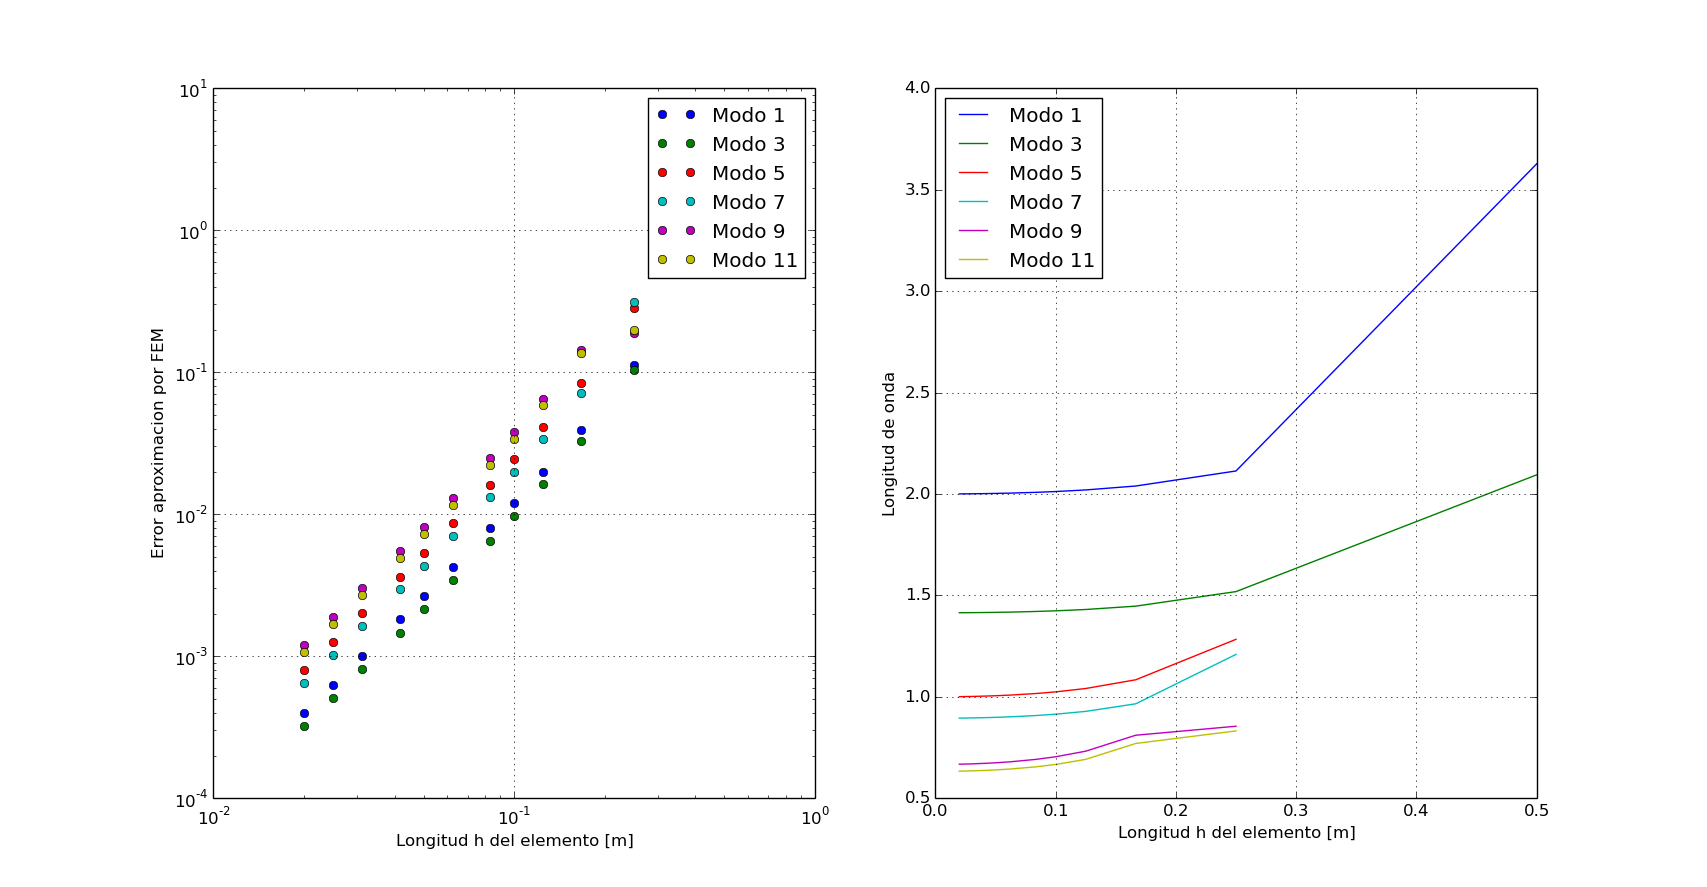
\includegraphics[width=17cm]{figuras/valores_propiosFEM.png}
  \caption{ Resultados aproximaci\'on valores propios mediante FEM y errores asociados}  
  \label{fig:velores_propios}
\end{figure}

Ajustando una curva a los datos ($log(E)$, $log(h)$) se obtiene una recta $log(E) = log(C) + p log(h)$ donde p es la taza de convergencia


\begin{table}[h]
\centering
\begin{tabular}{|c|c|c|}
\hline 
Modo & C & p \\ 
\hline 
1 & 0.62007961 & 2.4403783 \\
\hline 
3 & 0.39830035 & 2.33894099 \\ 
\hline 
5 & 0.69813644 & 2.26494859 \\  
\hline 
7 & 0.71017628 & 2.33846474 \\ 
\hline 
9 & 0.68486822 & 2.12311422 \\  
\hline 
11 &  0.70325574 & 2.17136287 \\
\hline 
\end{tabular} 
\caption{\hilight{Coeficientes de ajuste de las curvas $\log(E_\lambda)=\log(C)+p\log(h)$}}
\end{table}

Para el caso de la convergencia de los \hilight{vectores propios}, los resultados se muestran en la figura \ref{fig:vectores_propios}

\begin{figure}
  \centering
  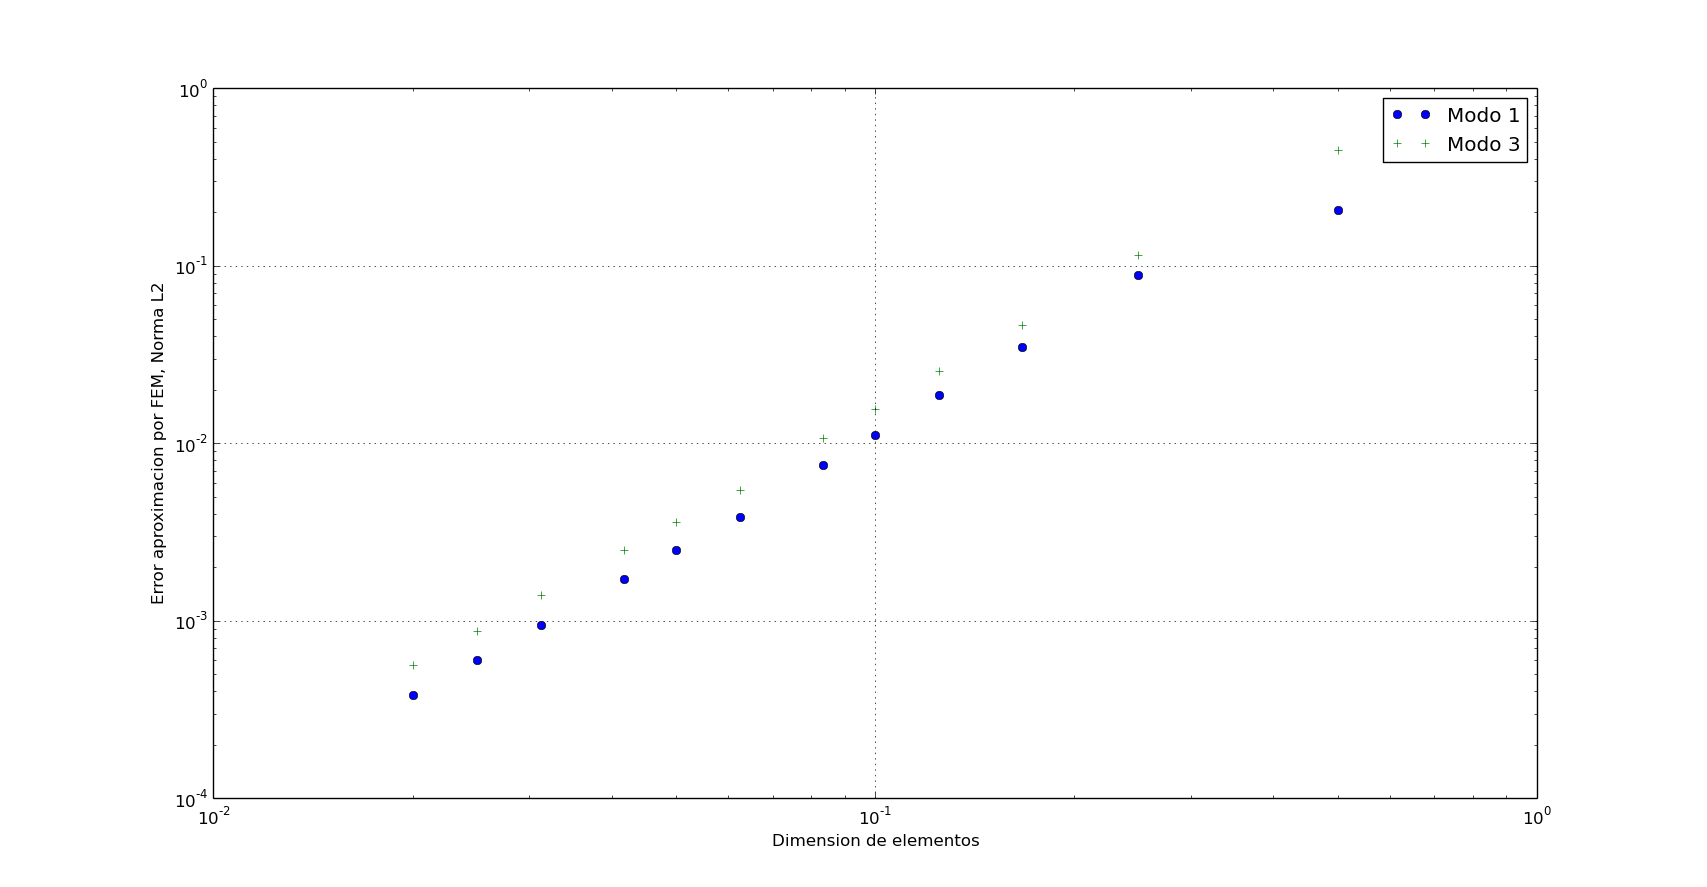
\includegraphics[width=17cm]{figuras/vectores_propiosFEM.png}
  \caption{ \hilight{Errores en norma $\mathcal{L}^2$ de los vectores asociados a cada modo propio}  }
  \label{fig:vectores_propios}
\end{figure}

Ajustando una recta a los datos ($log(E)$, $log(h)$)
\begin{table}[h]
  \centering
  \begin{tabular}{|c|c|c|}
  \hline 
  Modo & C & p \\ 
  \hline 
  1 & 0.0765871 & 2.04894336 \\  
  \hline 
  3 & 0.29036431 & 2.09300275 \\  
  \hline 
  \end{tabular} 
  \caption{\hilight{Coeficientes de ajuste de las curvas $\log(E_u)=\log(C)+p\log(h)$}}
\end{table}

En ambos casos se puede ver que la taza de convergencia es de orden 2.

\begin{figure}
  \centering
  \begin{subfigure}{0.3\textwidth}
    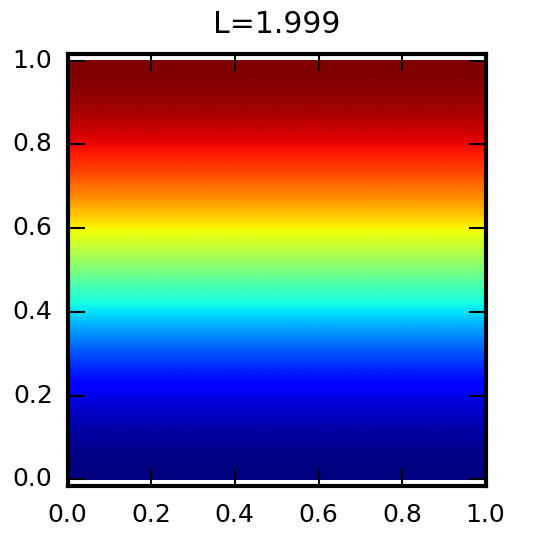
\includegraphics{figuras/modonum_1.png}
  \end{subfigure}
  ~
  \begin{subfigure}{0.3\textwidth}
    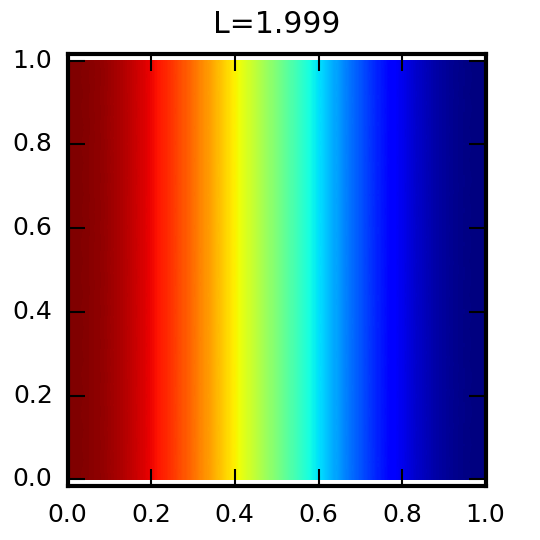
\includegraphics{figuras/modonum_2.png}
  \end{subfigure}
  
  \caption{Ejemplo de la multiplicidad de valores propios: modos de oscilaci\'on 1 y 2 usando $h=1/25$  mediante el m\'etodo de Elementos Finitos.}
\end{figure}

\begin{figure}  
  \centering
  \begin{subfigure}{0.4\textwidth}
    \centering
    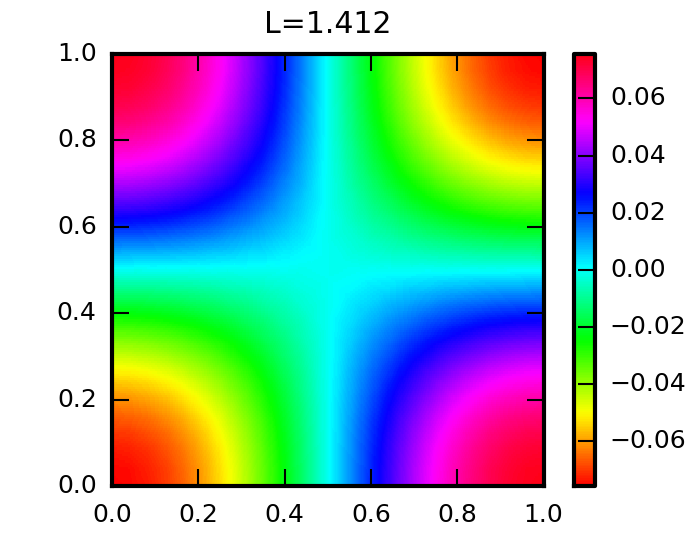
\includegraphics{figuras/modonum_3.png}
  \end{subfigure}
  ~
  \begin{subfigure}{0.4\textwidth}
    \centering
    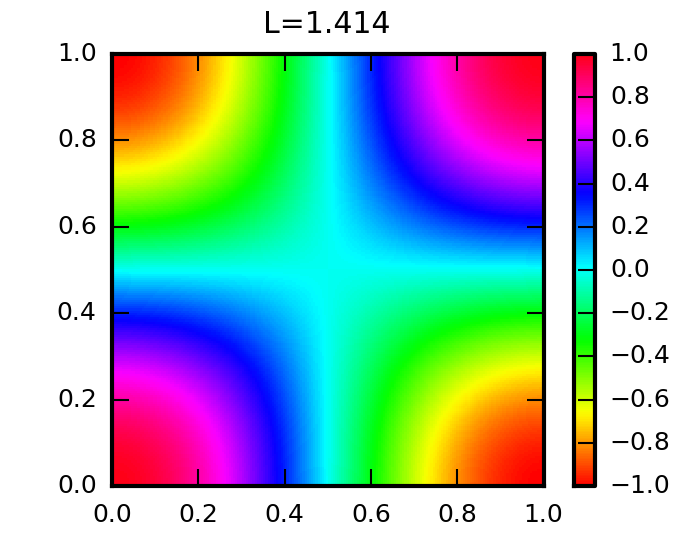
\includegraphics{figuras/modoanalitico_1_1.png}
  \end{subfigure}
  
  
  \begin{subfigure}{0.4\textwidth}
    \centering
    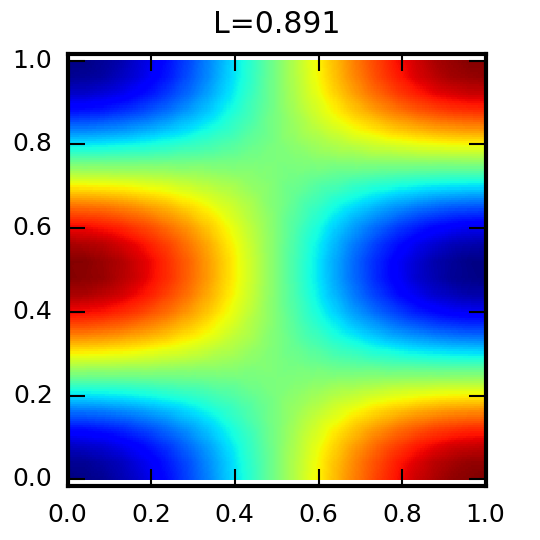
\includegraphics{figuras/modonum_6.png}
  \end{subfigure}
  ~
  \begin{subfigure}{0.4\textwidth}
    \centering
    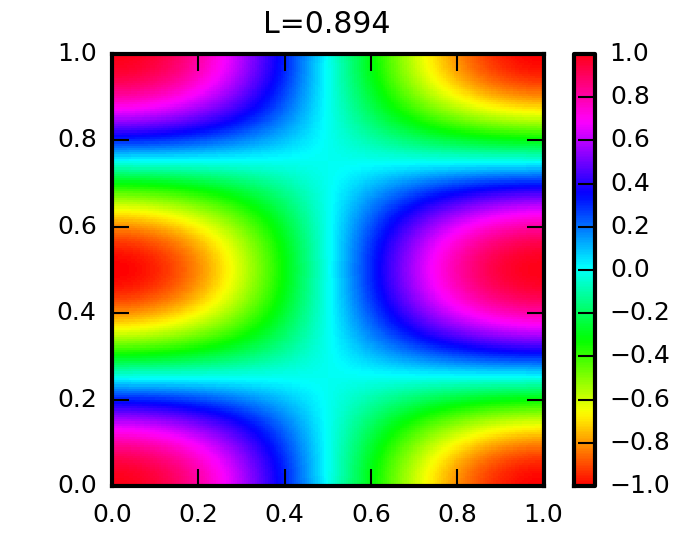
\includegraphics{figuras/modoanalitico_1_2.png}
  \end{subfigure}
  
  \caption{Modos de oscilaci\'on 3 y 6 obtenidos num\'ericamente para $h=1/25$ (primera columna) y mediante la soluci\'on anal\'itica para $(n,m)=(1,1)$ y $(n,m)=(1,2)$ (segunda columna)}
\end{figure}


  %\section{An\'alisis de resultados}
  %  asfadsf
un resultado muy bac\'an
  %\section{Conclusi\'on}
  %  adsfasf

  \pagebreak

  \twocolumn
  \begin{center}
	  {\bf C\'odigos de Python}
  \end{center}

  
%   \lstinputlisting[language=Python]{./codes/p1.py}
% % %   \pagebreak
%   \lstinputlisting[language=Python]{./codes/p2.py}
% %   \pagebreak
%   \lstinputlisting[language=Python]{./codes/tri3poisson.py}
% %   \pagebreak
%   \lstinputlisting[language=Python]{./codes/t8.py}
%   \pagebreak
%   \lstinputlisting[language=Python]{./codes/func_t6.py}
  
%   \lstinputlisting[language=Python]{./codes/func.py}
  
\end{document}
